\documentclass{article}
\usepackage[margin=1in]{geometry}

\usepackage{graphicx, subcaption}
\usepackage{amsmath}
\input{mytheme_listings}

\title{Calculating Farfields from Current Data}
\author{Aiden Incheol Jung}
\date{
	Department of Electric and Computer Engineering
	\today
}

\begin{document}

\maketitle

\section{Introduction}
This code intends to compute monostatic farfields from the mesh and electric/magnetic current data. All the data structure follows that of VWT-IE-Solver.

\section{Theory}
Monostatic farfields are computed using reciprocity theorem. Specifically, adjacent measurment is used. The process follows:
\begin{itemize}
	\item Place a vertical (VV) and horizontal (HH) plane wave source at the angle of incidence ($\theta$ and $\phi$).
	\item Use reciprocity to compute monostatic farfields: surface integral of the product of surface current and fields from the source.
\end{itemize}
\[ \mathbf{E}_\mathrm{sca}(\theta, \phi) = - j\omega \iint_S {\mathbf{J}(\mathbf{r}) \cdot \mathbf{E}^\mathrm{inc}_{\theta,\phi}(\mathbf{r}) dS } - jk \iint_S {\mathbf{M}(\mathbf{r}) \cdot \mathbf{H}^\mathrm{inc}_{\theta,\phi}(\mathbf{r}) dS } \]

\section{Usage}
All the input files must be in the same working path. The input files follow:
\begin{itemize}
	\item Mesh file (\texttt{.tri})
	\item In file (\texttt{.in})
	\item Current data (\texttt{.curJ}, \texttt{.curM})
\end{itemize}
e.g., 
\begin{lstlisting}[]
NAME.tri
NAME.in
NAME_Inc#1.curJ
NAME_Inc#1.curM
NAME_Inc#2.curJ
NAME_Inc#2.curM
...
\end{lstlisting}

\noindent
And then run the code:
\begin{lstlisting}[language=bash]
calc_efar.x NAME
\end{lstlisting}
where \texttt{NAME} is the name of the input files.


\section {Example: Cobra Duct cavity}
\begin{figure}
	\centering
	\begin{subfigure}{0.48\linewidth}
		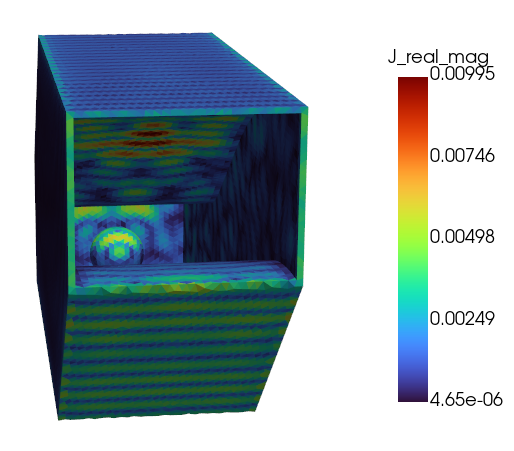
\includegraphics[width=\linewidth]{example/Inc1_J_real_mag.png}
		\caption{$J_\mathrm{real}$ at $\phi=0$ DEG}
	\end{subfigure}
	\hfill
	\begin{subfigure}{0.48\linewidth}
		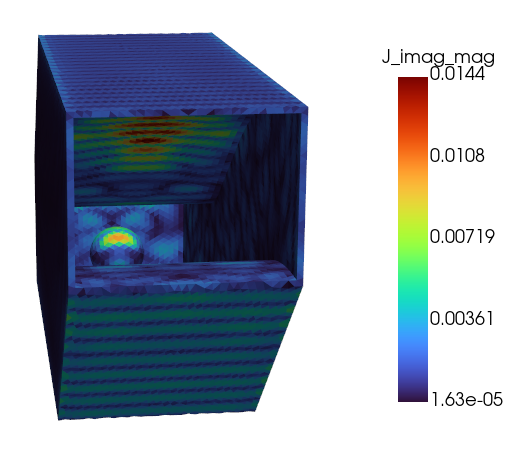
\includegraphics[width=\linewidth]{example/Inc1_J_imag_mag.png}
		\caption{$J_\mathrm{imag}$ at $\phi=0$ DEG}
	\end{subfigure}
	\vspace{3mm}
	\begin{subfigure}{0.48\linewidth}
		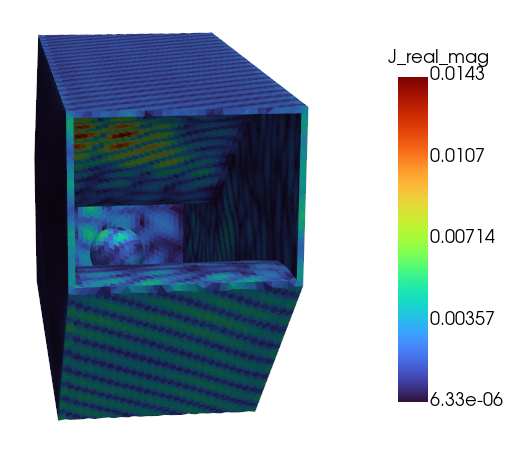
\includegraphics[width=\linewidth]{example/Inc10_J_real_mag.png}
		\caption{$J_\mathrm{real}$ at $\phi=30$ DEG}
	\end{subfigure}
	\hfill
	\begin{subfigure}{0.48\linewidth}
		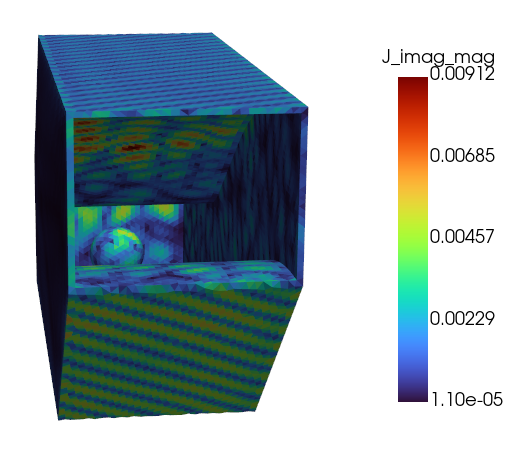
\includegraphics[width=\linewidth]{example/Inc10_J_imag_mag.png}
		\caption{$J_\mathrm{imag}$ at $\phi=30$ DEG}
	\end{subfigure}
	\vspace{3mm}
	\begin{subfigure}{0.9\linewidth}
		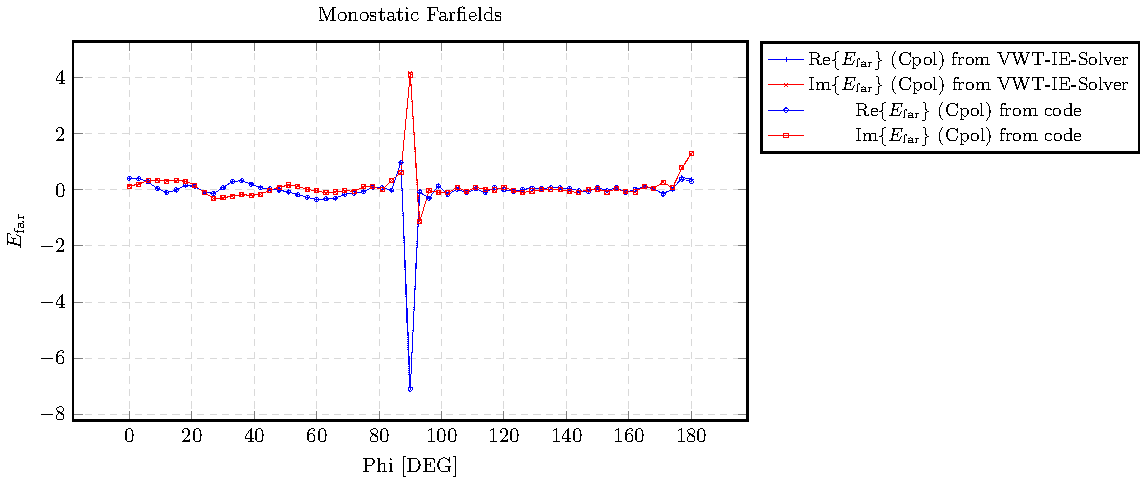
\includegraphics[width=\linewidth]{example/plot.pdf}
	\caption{Comparison of EFAR from \texttt{VWT-IE-Solver} and from \texttt{calc\_efar}}
	\end{subfigure}
\end{figure}

\end{document}
